\documentclass[10pt]{article}

\usepackage{graphicx}
\usepackage{amsmath}
\usepackage[utf8]{inputenc}
\usepackage[spanish]{babel}
\usepackage[vmargin=4cm,hmargin=4cm,letterpaper]{geometry}
\usepackage{color}
\usepackage{framed}
\usepackage{hyperref}

\usepackage{listings}
\definecolor{red}{RGB}{219,0,0}
\definecolor{pink}{RGB}{255,100,100}
\definecolor{gray}{RGB}{100,100,100}
\lstset{
		basicstyle=\ttfamily,
		frame=single,
		keywordstyle=\color{red},
		commentstyle=\color{gray},
		stringstyle=\color{pink},
		tabsize=3,
		language=verilog,
		backgroundcolor=\color{white}}

\usepackage{fancyhdr} 
\pagestyle{fancy}
\usepackage{lastpage}
\lhead{Laboratorio 1}
\chead{}
\rhead{Bitácora}
\lfoot{}
\cfoot{}
\rfoot{\footnotesize Page \thepage\ of \pageref{LastPage}}

\renewcommand{\headrulewidth}{0.4pt} 
\renewcommand{\footrulewidth}{0.4pt} 

\graphicspath{{./media/}}	%%multimedia path
\setlength{\parindent}{0pt}
%%*************************************************************************
\begin{document}

\begin{huge}
\begin{center}
\textbf{Laboratorio 1: Introducción\\ (Bitacora)}
\end{center}
\end{huge}

\begin{Large}
\begin{center}
Jose Apú (B10407), Francisco Molina (B12345), Marco Montero (A94000), Dennis Vargas (B16831)
\end{center}
\end{Large}

\section*{Ejercicio 1}
Del archivo Module\_ROM.v , se sustituye la linea:
\begin{lstlisting}
3: oInstruction = {`STO, `R4,16'd65000};
\end{lstlisting}
por:
\begin{lstlisting}
3: oInstruction = {`STO, `R4,16'd650};
\end{lstlisting}

Esto se debe a que esta instrución maneja un ciclo que depende del contenido del registro R4. Al ser mayor, mayor serán las repeticiones del ciclo.

\section*{Ejercicio 2}
Se debe añadir un método 'Sub que permita realizar un resta y observar el resultado de la resta en los leds.
Para esto se añadió al código minialu.v el siguiente código:
\begin{lstlisting}
`SUB:
	begin
		rFFLedEN     <= 1'b0;
		rBranchTaken <= 1'b0;
		rWriteEnable <= 1'b1;
		rResult      <= wSourceData1 - wSourceData0;
	end
\end{lstlisting}
Esto permite invocar el método desde el modulo Rom y asì usarlo como una instrucción de la alu.\\

A pesar de haber implementado la resta de la forma A - B. A la hora de diseñar se utiliza de la forma A + B1, donde B1 es el complemento en base 2 de B. Es mejor solo tener un bloque sumador , que dos bloques sumadores. Esto por que a la hora de sintetizar genera más compuertas el tener más bloques. En el diagrama \ref{diagrama_sumador} se observa la manera de implementarlo, se utiliza un mux, donde existe una linea de selección que permite que pase sí o no el complemneto a dos.\\ 

En la figura \ref{prueba_restador} se observa como ahora en lugar de sumar 1, resta 1. Lo que forma un contador descendente. De esta forma se logra probar el módulo restador (SUB).

\begin{figure}[hbtp]
\centering
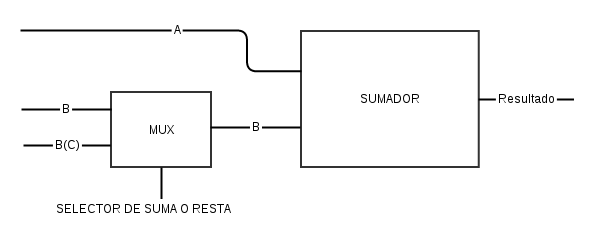
\includegraphics[width=1\textwidth]{sumador.png}
\caption{Diagrama de un sumador}
\label{diagrama_sumador}
\end{figure}



\begin{figure}[hbtp]
\centering
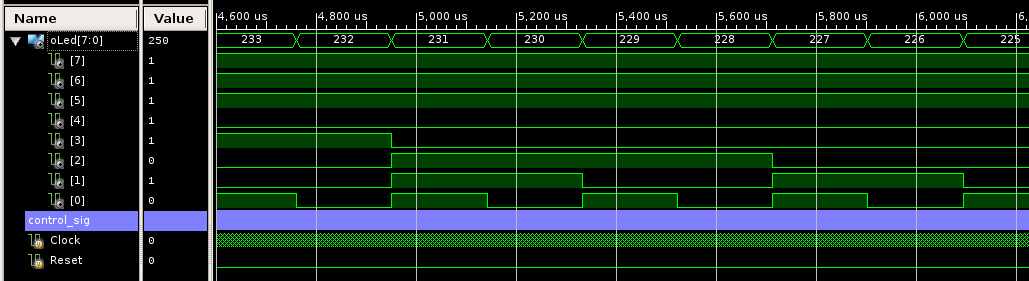
\includegraphics[width=1\textwidth]{restador.png}
\caption{Verificación del módulo restador}
\label{prueba_restador}
\end{figure}

\section*{Ejercicio 3}

En la figura \ref{raw_malo} se observa que cuando se lee la instrucción 6 (SUB), SourceData1 es 0, pero en realidad no lo es. Ya que este debe ser 6 por una instrucción anterior. De esta manera el pipeline tiene un hazar de read after write.

\begin{figure}[hbtp]
\centering
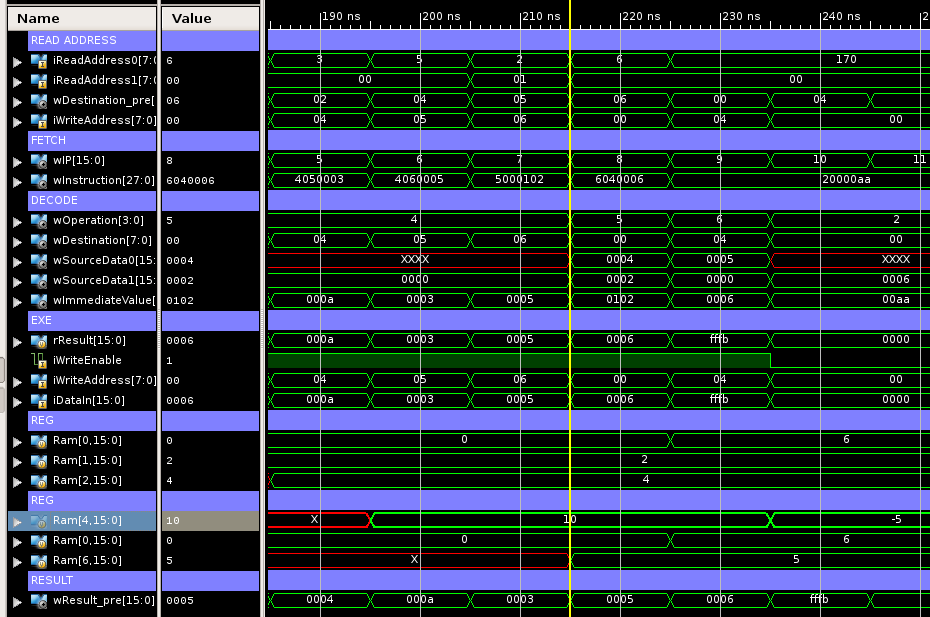
\includegraphics[width=1\textwidth]{read-write-malo.png}
\caption{}
\label{raw_malo}
\end{figure}

Para solucionarlo se utilizan dos muxes como se describen en las siguientes dos lineas de código:

\begin{lstlisting}
assign wSourceData0 = ( wSourceAddr0 == wDestination_pre) ?
wResult_pre :  wSourceData0_FromRam;

assign wSourceData1 = ( wSourceAddr1 == wDestination_pre) ?
wResult_pre : wSourceData1_FromRam;
\end{lstlisting}

Ahora, con la figura \ref{raw_bno} Si se observa que el SourceData1 no es 0, si no es 6, que fue el resultado de la suma anteior. De esta manera se logra determinar que corregimos el hazard de read after write para esta operación.

\begin{figure}[hbtp]
\centering
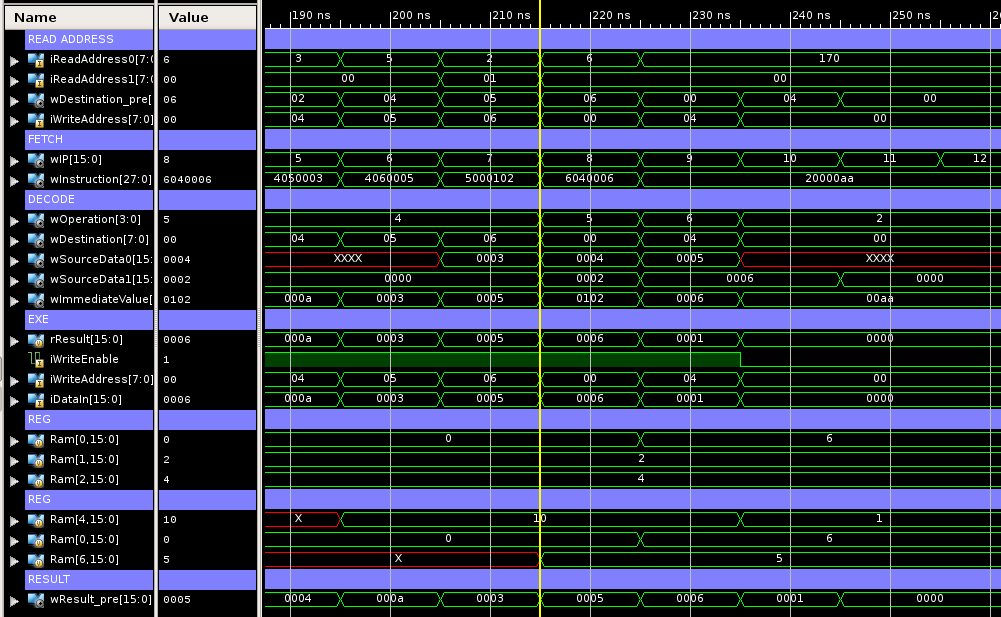
\includegraphics[width=1\textwidth]{read-write-bno.png}
\caption{}
\label{raw_bno}
\end{figure}

\pagebreak 

\section*{Ejercicio 4}
Los warnings que se presentan son debido a que no hay una asignación correcta en el tamaño de datos que ingresan a algunos puertos, por ejemplo, hay buses de datos de datos de 32 bits conectados a puertos de 16 bits y no se especifica cuales el rango de datos que ingresan por lo que por default se toman los primeros 16 bits del bus de datos. 
La solución a estos warnings es asignar un tamaño adecuado de los datos que ingresan a los puertos.
 
\end{document}
%%*************************************************************************
